\textbf{{1.HDLC协议的基本特点}}

{高级数据链路控制(HDLC)协议是ISO制定的{\textbf{面向比特}}(PPP是面向字节的,这个要记住)的数据链路控制协议。它可适用于链路的两种基本配置:非平衡配置和平衡配置。}

{a. 非平衡配置的特点是\textbf{由一个主站控制整个链路的工作};}

{b.
平衡配置的特点是\textbf{链路两端的两个站都是复合站,每个复合站都可以平等地发起数据传输,而不需要得到对方复合站的允许}。}

\textbf{{2.HDLC协议的帧格式}}

当采用HDLC协议时,从网络层交下来的分组,变成了HDLC协议帧的数据部分,数据链路层在信息字段的头尾各加上24位控制信息,这样就构成了一个完整的HDLC协议帧,如下图所示。

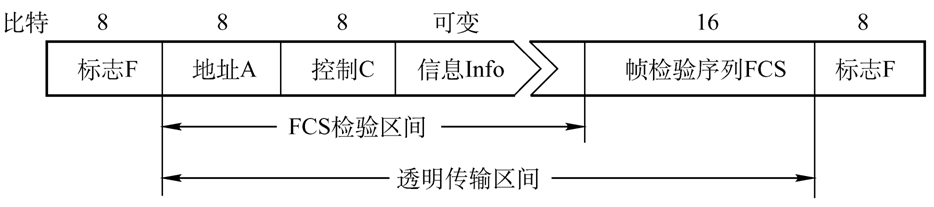
\includegraphics[width=3.33333in,height=0.73958in]{png-jpeg-pics/C2E8D187B3C55AEC1CDD2367ED1EB03B.png}

\textbf{1)标志字段(F)。}占8位,为``01111110'',首尾各有一个``0''作为帧的边界。为防止在两个标志字段F之间出现``01111110'',HDLC使用比特填充的首尾标志法。当一串比特流未加上控制信息时,扫描整个帧,只要发现有5个连续``1'',就立即填入一个``0''。

\textbf{2)地址字段(A)。}占8位。若使用非平衡方式传送数据,为次站的地址;若使用平衡方式传送数据,为确认站的地址。全``1''为广播方式,全``0''为无效地址。

\textbf{3)控制字段(C)。}占8位。最复杂的字段,HDLC的许多重要功能都靠控制字段实现。根据其最前面两位的取值,可将HDLC帧划分为三类:信息帧(I帧)、监督帧(S帧)和无编号帧(U帧)。

{\textbf{提醒:三类帧的记忆方式,每当看到HDLC帧的分类就想到``无监息''=``无奸细''。}}

信息帧用来传输数据信息,或使用捎带技术对数据进行确认和应答;监督帧用于流量控制和差错控制,执行对信息帧的确认、请求重发和请求暂停发送等功能;无编号帧用于提供对链路的建立、拆除以及多种控制功能。

\textbf{4)信息字段。}长度任意,存放来自网络层的协议数据单元。

\textbf{5)帧检验序列(FCS)。}占16位,即循环冗余码检验中的冗余码。检验区间包括地址字段、控制字段和信息字段。
